\documentclass{article}
\usepackage{tikz}
\usepackage{amsmath}
\usepackage{caption}
\usepackage{graphicx} % 加载图形包用于缩放
\usetikzlibrary{decorations.pathreplacing} % 加载括号装饰库
\pagestyle{empty}

\begin{document}

    \begin{figure}[htbp]
        \centering
        \captionsetup{type=figure} % 不显示标题
        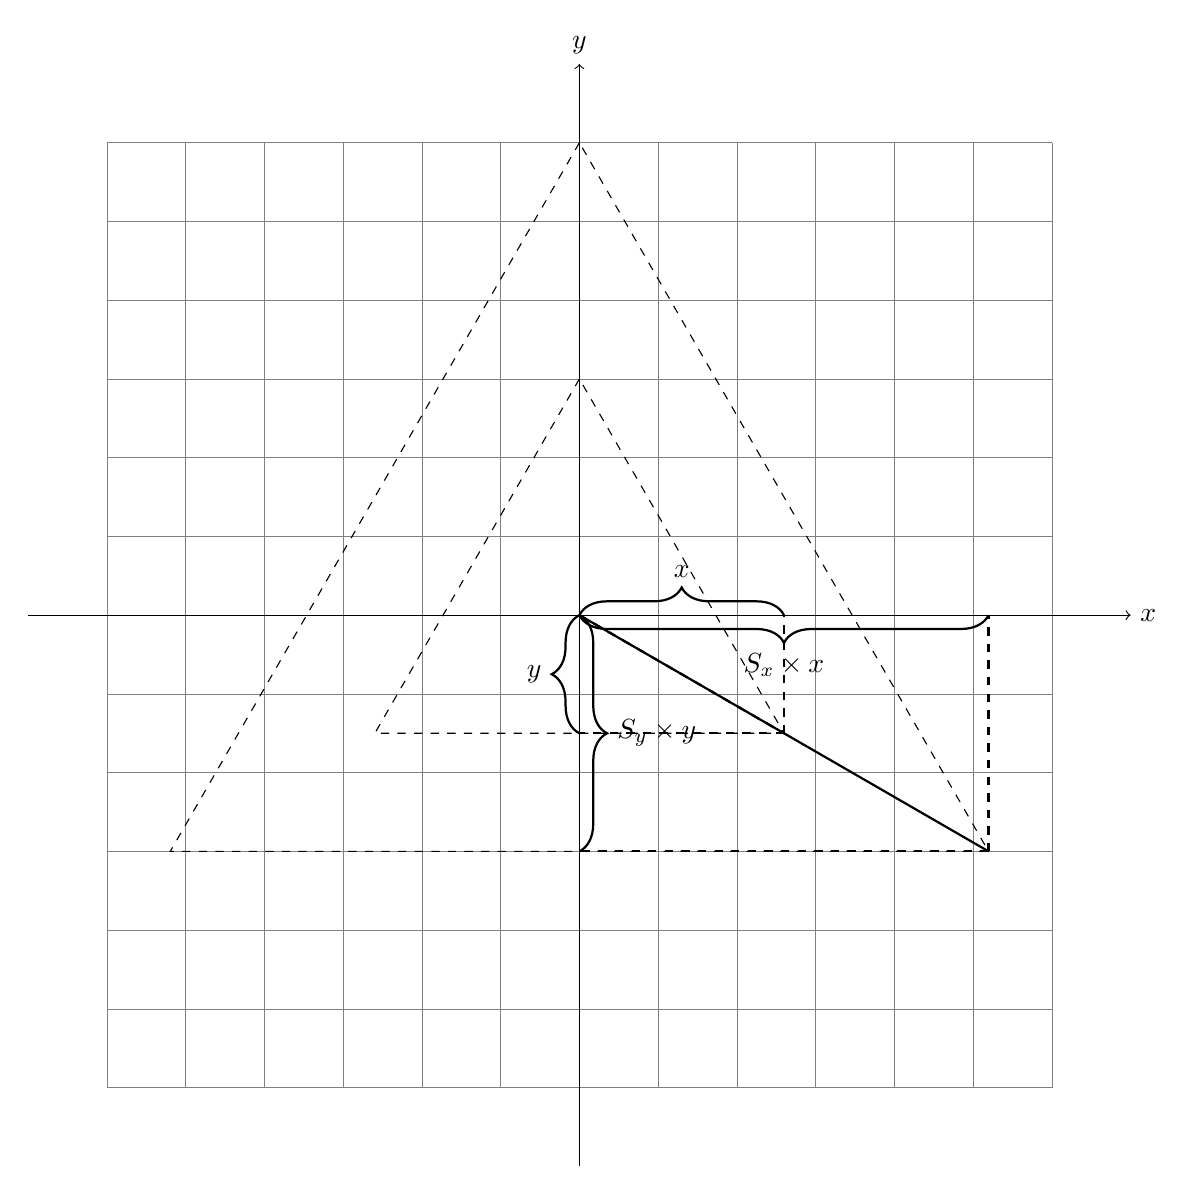
\begin{tikzpicture}
            \draw[very thin, gray] (-6,-6) grid (6,6);
            % 绘制等边三角形
            \draw[thin, dashed] (90:3) -- (210:3) -- (330:3) -- cycle; % 顶点角度依次是 60, 180, 300 度
            \draw[thin, dashed] (90:6) -- (210:6) -- (330:6) -- cycle; % 顶点角度依次是 60, 180, 300 度

            \coordinate (x) at (330:3 |- 0,0);
            \coordinate (y) at (330:3 -| 0,0);
            \coordinate (x') at (330:6 |- 0,0);
            \coordinate (y') at (330:6 -| 0,0);

            \draw[thick, dashed] (330:3) -- (x);
            \draw[thick, dashed] (330:3) -- (y);
            \draw[thick, dashed] (330:6) -- (x');
            \draw[thick, dashed] (330:6) -- (y');

%            \node at (x) [above right] {$P_x$};
%            \node at (y) [above right] {$P_y$};
%            \node at (x') [above right] {$P_{x'}$};
%            \node at (y') [above right] {${P_{y'}}$};

            % 标记顶点
%            \node at (90:3) [above right] {$A$};
%            \node at (210:3) [below left] {$B$};
%            \node at (330:3) [below right] {$C$};
%
%            \node at (90:6) [above right] {$A'$};
%            \node at (210:6) [below left] {$B'$};
%            \node at (330:6) [below right] {$C'$};

            % 绘制从原点到 A 点的线段
            \draw[thick] (0,0) -- (330:6);
            \draw[thick, dashed] (0,0) -- (330:3);

            % 绘制坐标轴
            \draw[->] (-7,0) -- (7,0) node[right] {$x$};
            \draw[->] (0,-7) -- (0,7) node[above] {$y$};

%            % 标记长度 l
%            \draw[thick, decorate,dashed, decoration={brace, amplitude=10pt}]
%            (0, 0) -- (330:3) node[midway, right=10pt, above=5pt] {$l$};
%
%            % 标记长度 S x l
%            \draw[thick, decorate, dashed, decoration={brace, amplitude=10pt, mirror}]
%            (0, 0) -- (330:6) node[midway, left=10pt, below=5pt] {$S \times l$};

            \draw[thick, decorate, decoration={brace, amplitude=10pt}]
            (0, 0) -- (x) node[midway, above=10pt] {$x$};

            \draw[thick, decorate, decoration={brace, amplitude=10pt, mirror}]
            (0, 0) -- (x') node[midway,  below=10pt] {$S_x \times x$};

            \draw[thick, decorate, decoration={brace, amplitude=10pt, mirror}]
            (0, 0) -- (y) node[midway, left=10pt] {$y$};

            \draw[thick, decorate, decoration={brace, amplitude=10pt, }]
            (0, 0) -- (y') node[midway,  right=10pt] {$S_y \times y$};


        \end{tikzpicture}
        \caption*{} % 不显示标题
        \label{fig:equilateral_triangle}
    \end{figure}

\end{document}
